\documentclass[11pt, a4paper, leqno]{article}
\usepackage{a4wide}
\usepackage[T1]{fontenc}
\usepackage[utf8]{inputenc}
\usepackage{float, afterpage, rotating, graphicx}
\usepackage{epstopdf}
\usepackage{longtable, booktabs, tabularx}
\usepackage{fancyvrb, moreverb, relsize}
\usepackage{eurosym, calc}
% \usepackage{chngcntr}
\usepackage{amsmath, amssymb, amsfonts, amsthm, bm}
\usepackage{caption}
\usepackage{mdwlist}
\usepackage{xfrac}
\usepackage{setspace}
\usepackage{xcolor}
\usepackage{subcaption}
\usepackage{minibox}
\usepackage{float}
% \usepackage{pdf14} % Enable for Manuscriptcentral -- can't handle pdf 1.5
% \usepackage{endfloat} % Enable to move tables / figures to the end. Useful for some submissions.


\usepackage[
    natbib=true,
    bibencoding=inputenc,
    bibstyle=authoryear-ibid,
    citestyle=authoryear-comp,
    maxcitenames=3,
    maxbibnames=10,
    useprefix=false,
    sortcites=true,
    backend=biber
]{biblatex}
\AtBeginDocument{\toggletrue{blx@useprefix}}
\AtBeginBibliography{\togglefalse{blx@useprefix}}
\setlength{\bibitemsep}{1.5ex}
\addbibresource{refs.bib}





\usepackage[unicode=true]{hyperref}
\hypersetup{
    colorlinks=true,
    linkcolor=black,
    anchorcolor=black,
    citecolor=black,
    filecolor=black,
    menucolor=black,
    runcolor=black,
    urlcolor=black
}


\widowpenalty=10000
\clubpenalty=10000

\setlength{\parskip}{1ex}
\setlength{\parindent}{0ex}
\setstretch{1.5}


\begin{document}

\title{Endogenous adjustment in behavior based on incidence of COVID-19: Evidence from the Netherlands
\thanks{Anum Mushtaq, Nitesh Shisodia, University of Bonn. Email: \href{mailto:s6anmush@uni-bonn.de}{\nolinkurl{s6anmush [at] uni-bonn [dot] de}}.}}

\author{Anum Mushtaq, Nitesh Shisodia}

\date{
    % {\bf Preliminary -- please do not quote}
    \\[1ex]
    \today
}

\maketitle


\begin{abstract}
This study aims to observe the relationship between CoViD-19 incidence value per hundred thousand population and contact reduction behavior of the individuals in Netherlands using LISS pan. This study can be very useful to the policymakers for identification of relevant behavior of general population to curb the spread of the virus. We expected that the individuals should increase the contact reduction behavior if they see rise in Covid-19 incidence value. Our results suggest so but cannot establish causal relation as they are prone to various limitations which are also discussed.
    
\end{abstract}
\clearpage

\section{Introduction} % (fold)
\label{sec:introduction}
The CoViD-19 pandemic was officially declared a Public Health Emergency of International Concern on January 30, 2020 and a global pandemic on March 11, 2020 by the World Health Organization (WHO). There is present extensive literature that emphasizes the unexpected nature of this global pandemic and the diverse consequences that it has brought forward upon societies. The  CoViD-19 pandemic affects societies at the core, causing human suffering, a rise in death rate and promotion of disconnectedness amongst members of a social group. In order to efficiently combat this virus countries have sought to control the transmission of this virus by imposing restrictions on population movement. Hence, encouraging the practice of strict social distancing and participating in quarantine measures to be able to reduce the number of contacts. These interventions were aimed to reduce the number of cases of CoViD-19 in the population measured efficiently by the incidence rate. The incidence rate is a measure of the frequency of the CoViD-19 pandemic over a specified period of time. With the passage of time, since this pandemic began, we have observed a reduction in human mobility in times when the incidence rate has been high. This can be explained through stricter social distancing policies implemented with higher incidence rates limiting social interaction amongst the population. 

In our study we attempt to empirically verify the association between the incidence rate for new cases in the Netherlands with respect to contact reduction behavior amongst individuals. According to our assumptions, we should observe a higher frequency of contact reduction behavior with a higher value incidence rate. We conduct our study using using LISS (Longitudinal Internet Studies for the Social Sciences) panel data. The LISS panel data is an internet based household panel administered by the centERdata (Tilburg University, The Netherlands). The questionnaires have been conducted to survey LISS panel participants concerning their experiences, expectations and their socioeconomic situation at the time of the CoViD-19 pandemic. The LISS panel data provides extensive surveys for each of the waves, with substantial documentation available from survey conduced in the first wave up to the seventh wave. However, to attain information exclusive to contact reduction behavior we have directed our focus on contact reduction factors from the first to the fifth wave. In our study we use contact reduction variables and contact reduction factors interchangeably. Furthermore, information related to the incidence rate for new cases has been collected from ``Our World in Data'', a scientific online publication focused on large global issues. 
 
In our study we study the association between the contact reduction behavior and the incidence rate in the Netherlands mostly through graphical representation. However, we have been unfortunate in attaining relevant contact reduction factors common within all the waves, apart from three factors consistent in the fourth to fifth wave, which proved the process of obtaining a precise estimation of the effect of contact reduction behavior on the incidence rate quite cumbersome. For these reasons, we provide an efficient graphical representation of a reduction in the incidence rate followed by a reduction in human mobility in the Netherlands using the average incidence rate for the month in which the LISS panel survey was collected representing quantitative and qualitative data regarding contact reduction for those participating in the survey. Due to the limitation stated above, we do not however graphically present a time series of the association between individual contact reduction variables and incidence rate in the Netherlands over a specified period of time. 

We further contribute to literature by applying an ordinary least squares statistical method to study the association between the average monthly incidence rate with respect to the contact reduction variables for a specific month and across all the waves, in addition we continue with performing the OLS by taking the logarithm of the incidence rate to  show relation between the change in new CoViD-19 cases incidence values and contact reduction  overtime. 







\section{Data Management}
The LISS panel data provides several variables related to contact reduction, these variables have been distributed amongst the first to fifth wave. In order to efficiently quantify the data, we have altered the data set to contain only boolean data types that coincide with our assumption concerning contact reduction behavior. According to our assumptions, a value of ``1.0'' has been assigned as a response to a question for the survey if the response corresponds to contact reduction, and a value of ``0.0'' if the response does not correspond to contact reduction. We have conducted the exact procedure with responses for the survey questions that were a string data type(qualitative). Here, we are documenting all the wave-wise variables and our assumptions. 

\subsection{Wave one}
This provides the documentation of the LISS panel questionnaire on the CoViD-19 pandemic for the first wave. This questionnaire was fielded between March 20, 2020 and March 31, 2020 and provides the relevant contact reduction variables. The variables identified consist of ``avoid\textunderscore busy\textunderscore places'',
``avoid\textunderscore public\textunderscore places'',
``maintain\textunderscore distance'', ``adjust\textunderscore school\textunderscore work'',  ``quarantine\textunderscore symptoms'',
``quarantine\textunderscore no\textunderscore symptoms'',``no\textunderscore avoidance\textunderscore behaviors'',``contact\textunderscore 

older\textunderscore people'' , this contact reduction factor contains responses in the form of strings which were replaced in the following manner; `none at all', `hardly any` and`some' have been assigned the value ``1.0'' whereas `a lot', `a whole lot' have been assigned the value ``0.0'', lastly, ``contact\textunderscore young\textunderscore people'',this contact reduction factor also contains responses in the form of strings which were replaced in the following manner;  `never' has been assigned the value of ``1.0'' whereas  
`once a week', `several times' and `every day' has been assigned the value ``0.0''.

\subsection{Wave two}
 This provides the documentation of the LISS Panel questionnaire on the CoViD-19 pandemic for wave two. This questionnaire was fielded in April 2020 and provides the relevant contact reduction variables.The variables identified consist of ``change\textunderscore contacts\textunderscore personal'', this contact reduction factor contains responses in the form of strings which were replaced in the following manner; `much less' and ‘less’ have been assigned the value ``1.0'', ‘roughly equal’, ‘more’ and ‘much more’ have been assigned the value  ``0.0'', ``change\textunderscore contacts\textunderscore distanced'',this contact reduction factor contains responses in the form of strings which were replaced in the following manner;  'much less' and `less' have been assigned the value ``0.0'' and `roughly equal', `more' and `much more' have been assigned the value of ``1.0''.

\subsection{Wave three}
This provides the documentation of the LISS Panel questionnaire on the CoViD-19 pandemic for wave three. This questionnaire was fielded in May 2020 and provides the relevant contact reduction variables.The variables identified consist of ``outside\textunderscore no", this variable identifies whether an individual has been outside, ``outside\textunderscore contacts'', this variable identifies whether an individual has had outside contacts in past week, ``outside\textunderscore garden'', this variable identifies whether an individual visited a garden within his/her own vicinity,``outside\textunderscore shopping'' , this variable identifies whether an individual has engaged in any shopping, ``outside\textunderscore purchases'', this variables identifies any outside purchases, ``outside\textunderscore care'', this variable identifies whether an individual has been outside for the provision of informal care, and lastly ``outside\textunderscore medical'', this variable identifies whether an individual has been outside for any medical reasons. 

\subsection{Wave four}
This provides the documentation of the LISS Panel questionnaire on the CoViD-19 pandemic for wave four.This questionnaire was fielded in June 2020 and provides the relevant contact reduction variables. The variables identified consist of ``avoid\textunderscore cafe", ``avoid\textunderscore theater'',``avoid\textunderscore 

public\textunderscore transport'', and ``avoid\textunderscore gym''. These variables identify whether an individual has partaken in any of the respective activities. These contact reduction factors contain responses in the form of strings which were replaced in the following manner; `before the outbreak, but not now' and `not before the outbreak and not now' have been assigned the value of ``1.0'' and `as often as before the outbreak',`much less often than before the outbreak',`much less often than before the outbreak',`a little less often than before the outbreak',`more often than before the outbreak' have been assigned the value of ``0.0''. 

\subsection{Wave five}
This provides the documentation of the LISS Panel questionnaire on the CoViD-19 pandemic for wave five. This questionnaire was fielded in September 2020 and provides the relevant contact reduction variables. The variables identified consist of The variables identified consist of ``avoid\textunderscore cafe", ``avoid\textunderscore theater'',``avoid\textunderscore public\textunderscore transport''. These contact reduction factors contain responses in the form of strings similar to wave four and hence were replaced in the exact manner.

\section{Factors of contact reduction}


In our study we have identified the relevant variables related to contact reduction for the five months March, April, May, June and September. These months represent the five waves documented by the LISS panel survey. 

In order to effectively estimate the association between the CoViD-19 incidence rate and factors related to contact reduction behavior we have calculated the average of these variables, which can be shown in figure 1. Figure 1, creates a bar plot for each variable with it's averages that ranges between ``0.0 - 1.0''. Due to the fact that there are a few variables common among the waves, we have created an additional bar plot to represent these common variables in Figure 2. Hence, figure 2 represents the average of the variables with an additional insight into the common variables between the fourth and the fifth wave.



\begin{figure}[H]
    \caption{Month-wise average of contact reduction variables}
    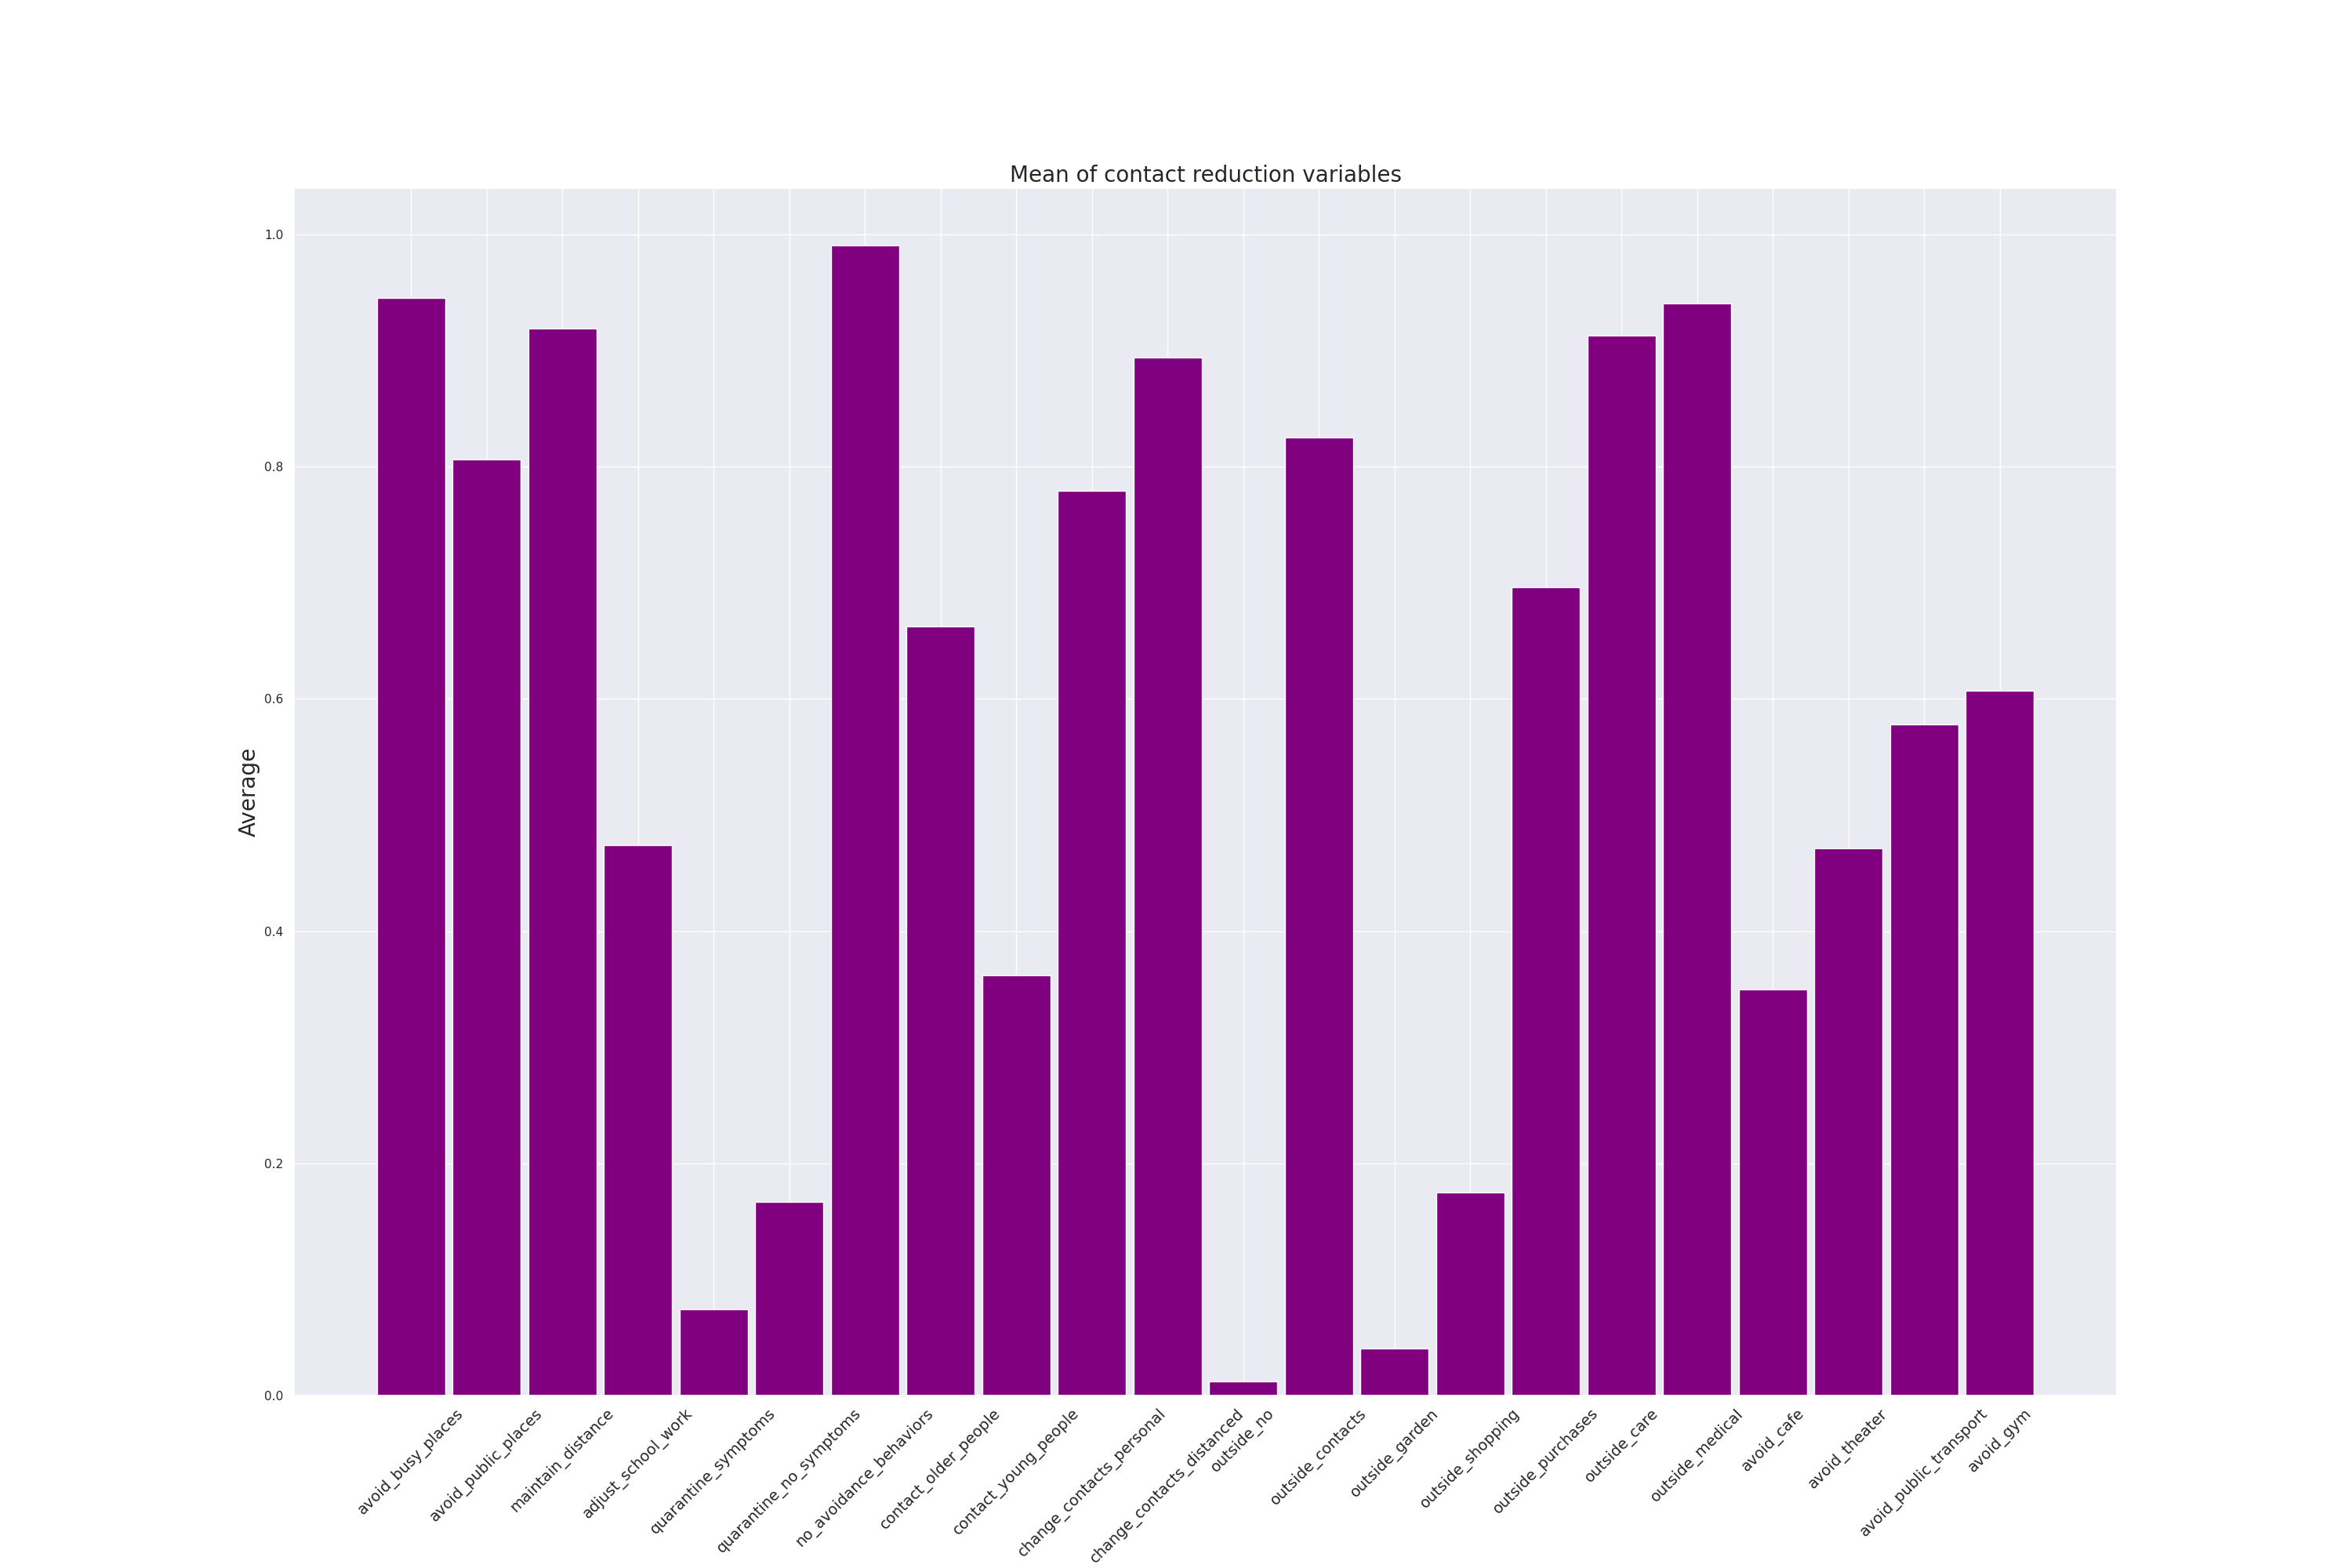
\includegraphics[width=\textwidth]{../../bld/figures/contact_reduction_variables}
\end{figure}

\begin{figure}[H]
    \caption{Factors of contact reduction}
    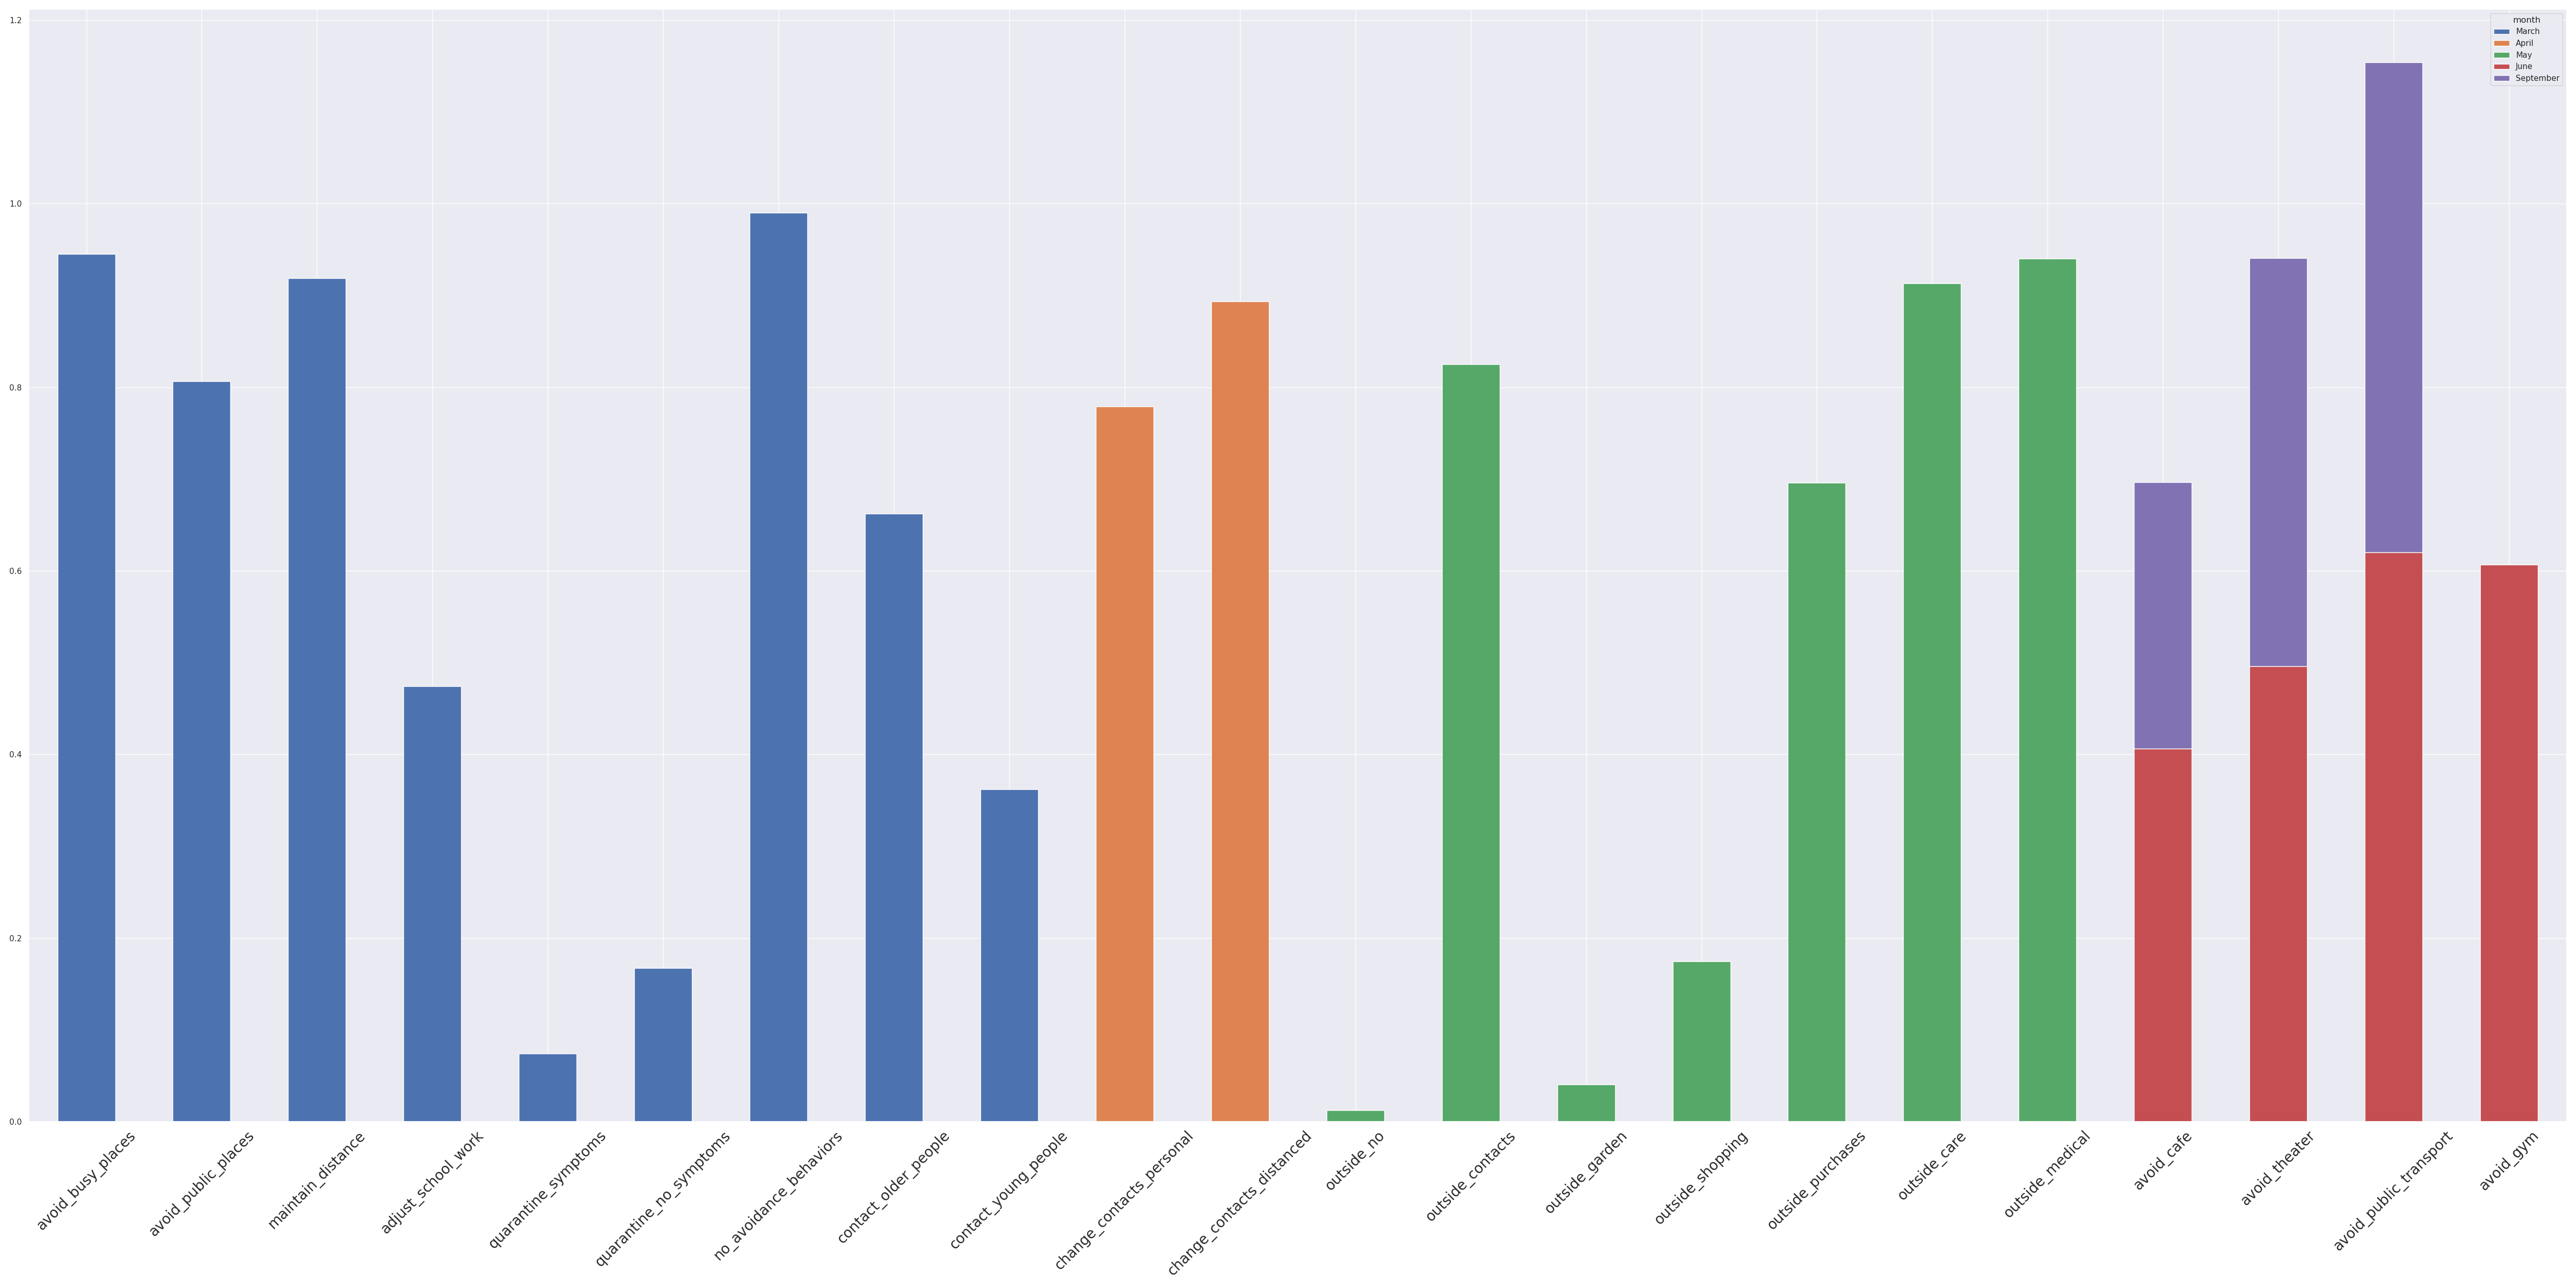
\includegraphics[width=\textwidth]{../../bld/figures/contact_reduction_variables_2}
\end{figure}
\begin{figure}[H]
    \caption{Common factors of contact reduction in wave four and five}
    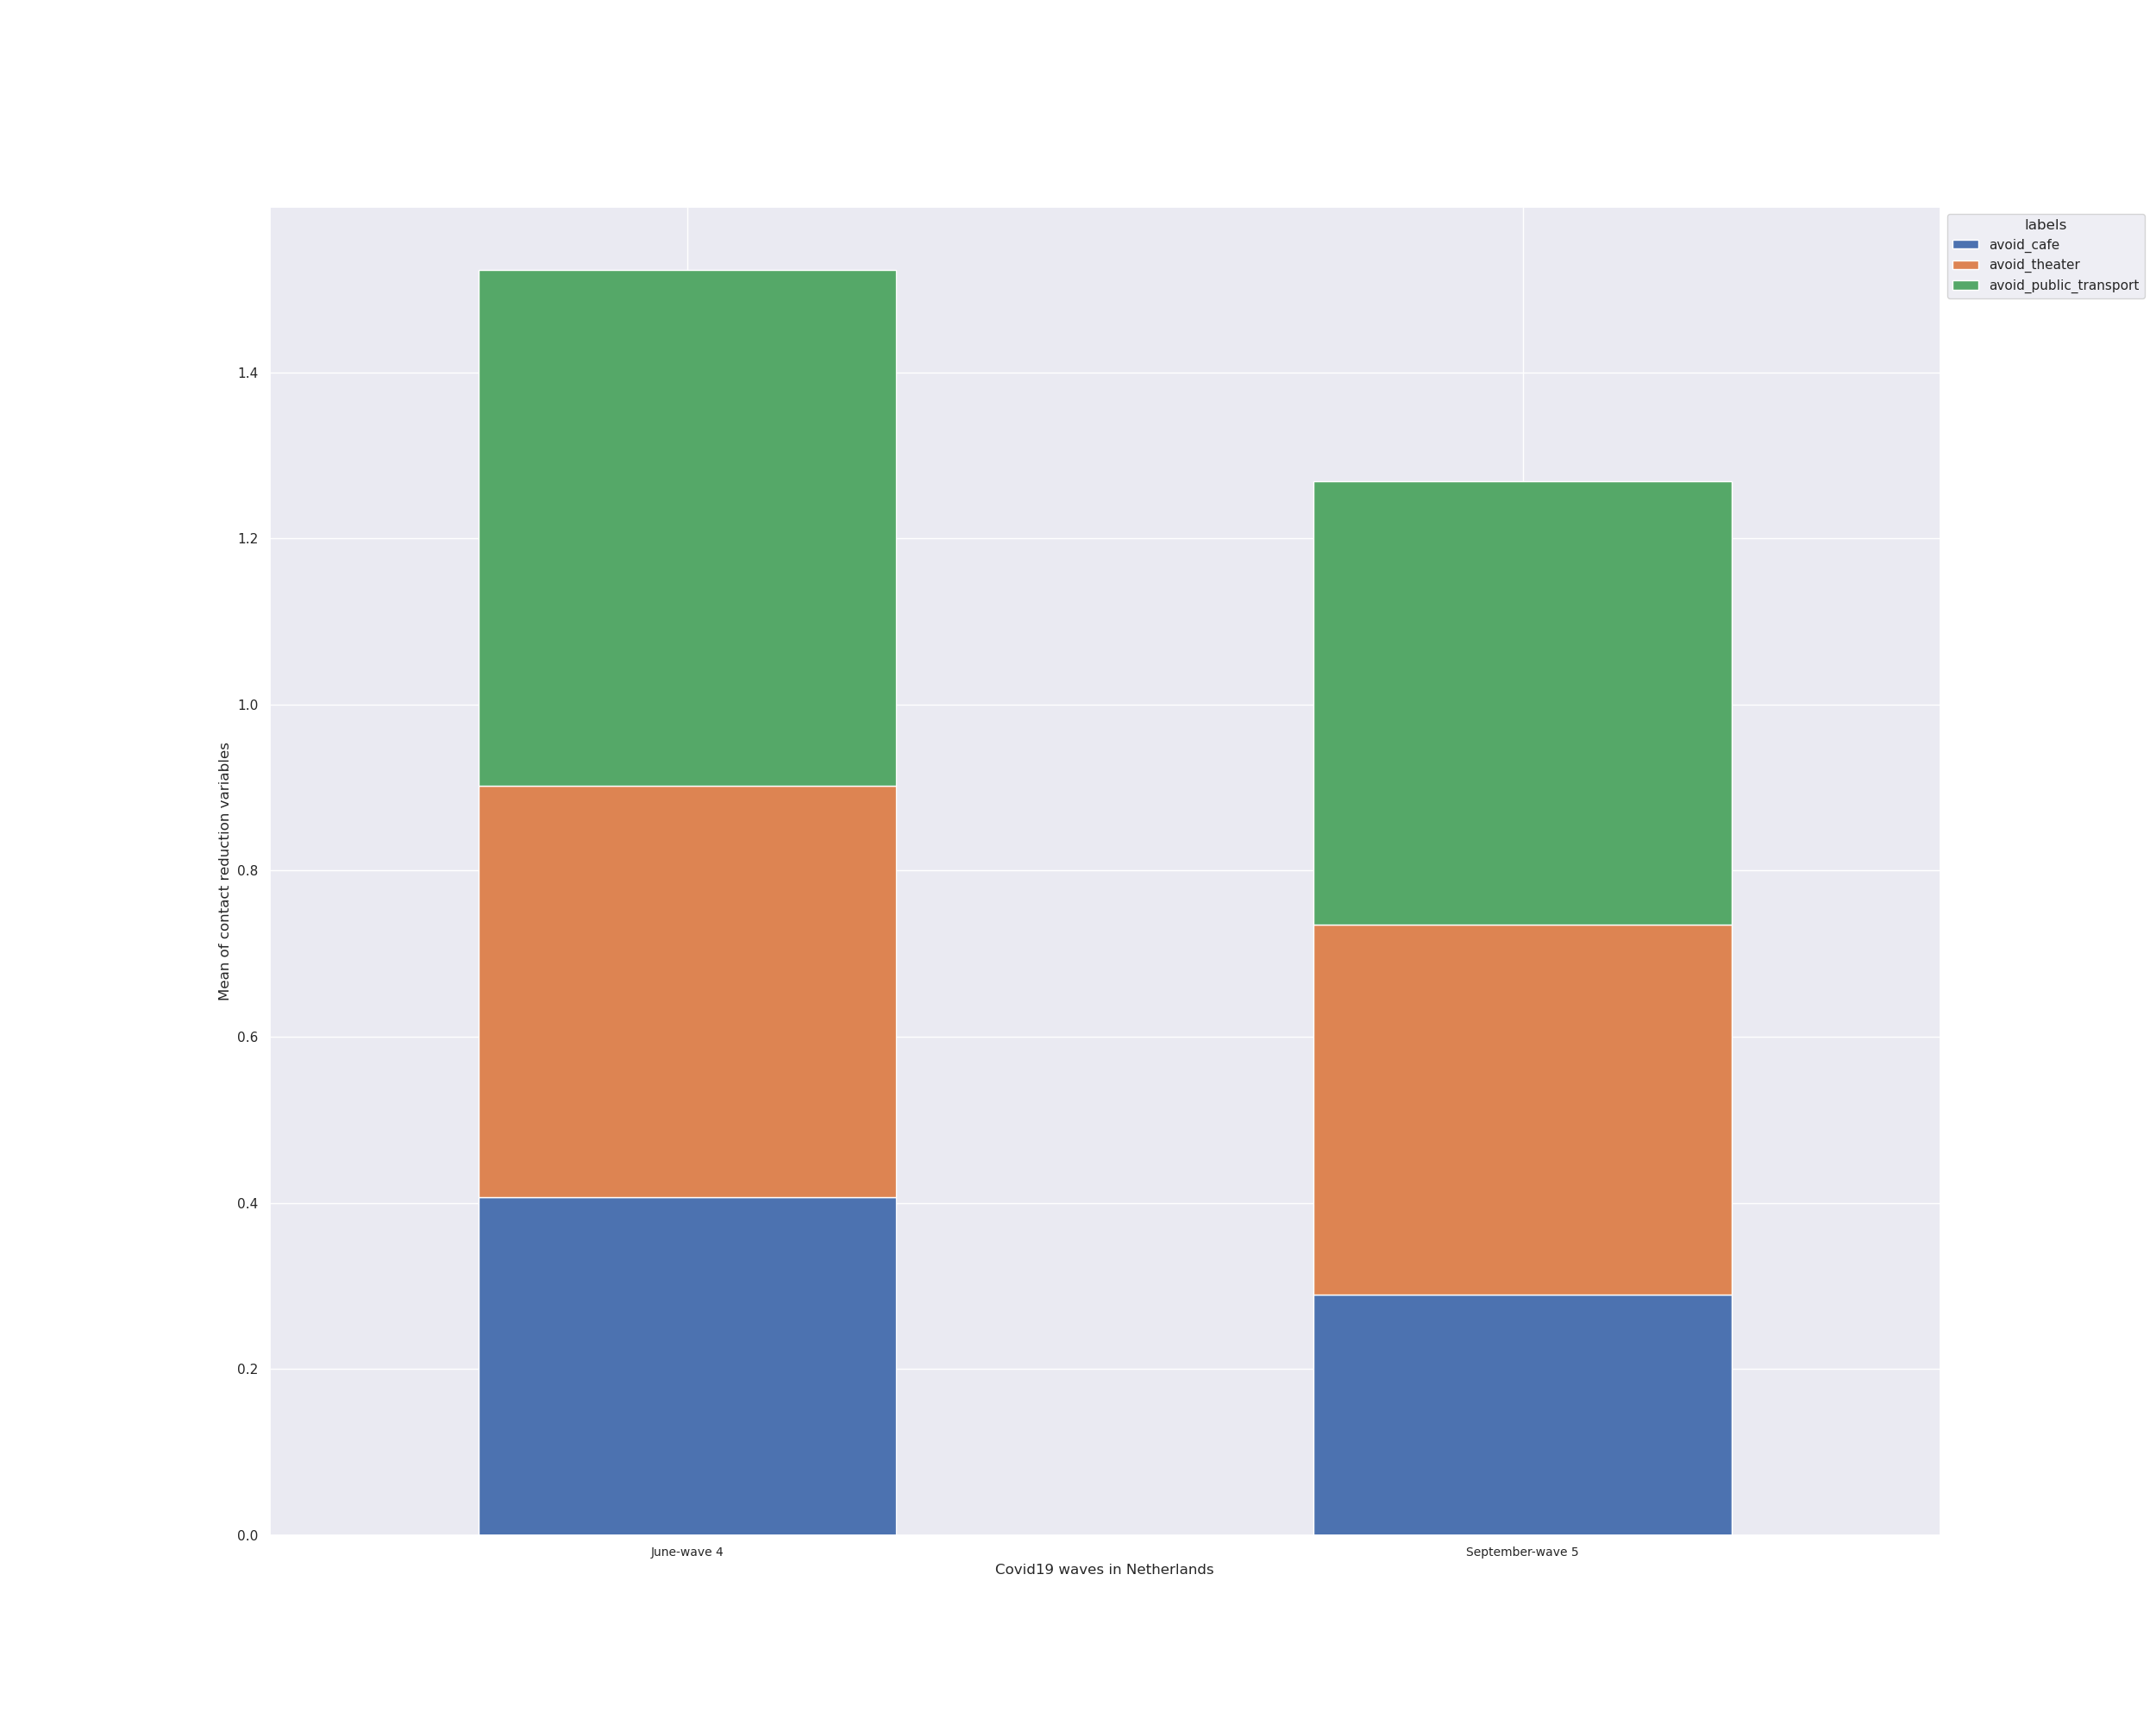
\includegraphics[width=\textwidth]{../../bld/figures/transition_wave4-_wave5}
\end{figure}
\pagebreak

\newpage

To gain further information regarding the contact reduction variables we attempt to graph these
variables in the month the survey was conducted. Figure 3 represents the month-wise average of these contact reduction variables with the standard deviation of these variables. Figure 4 on the other hand provides a distribution of the averages of these variables with the month of the LISS panel survey. 


\begin{figure}[H]
    \caption{Month-wise average of contact reduction variables}
    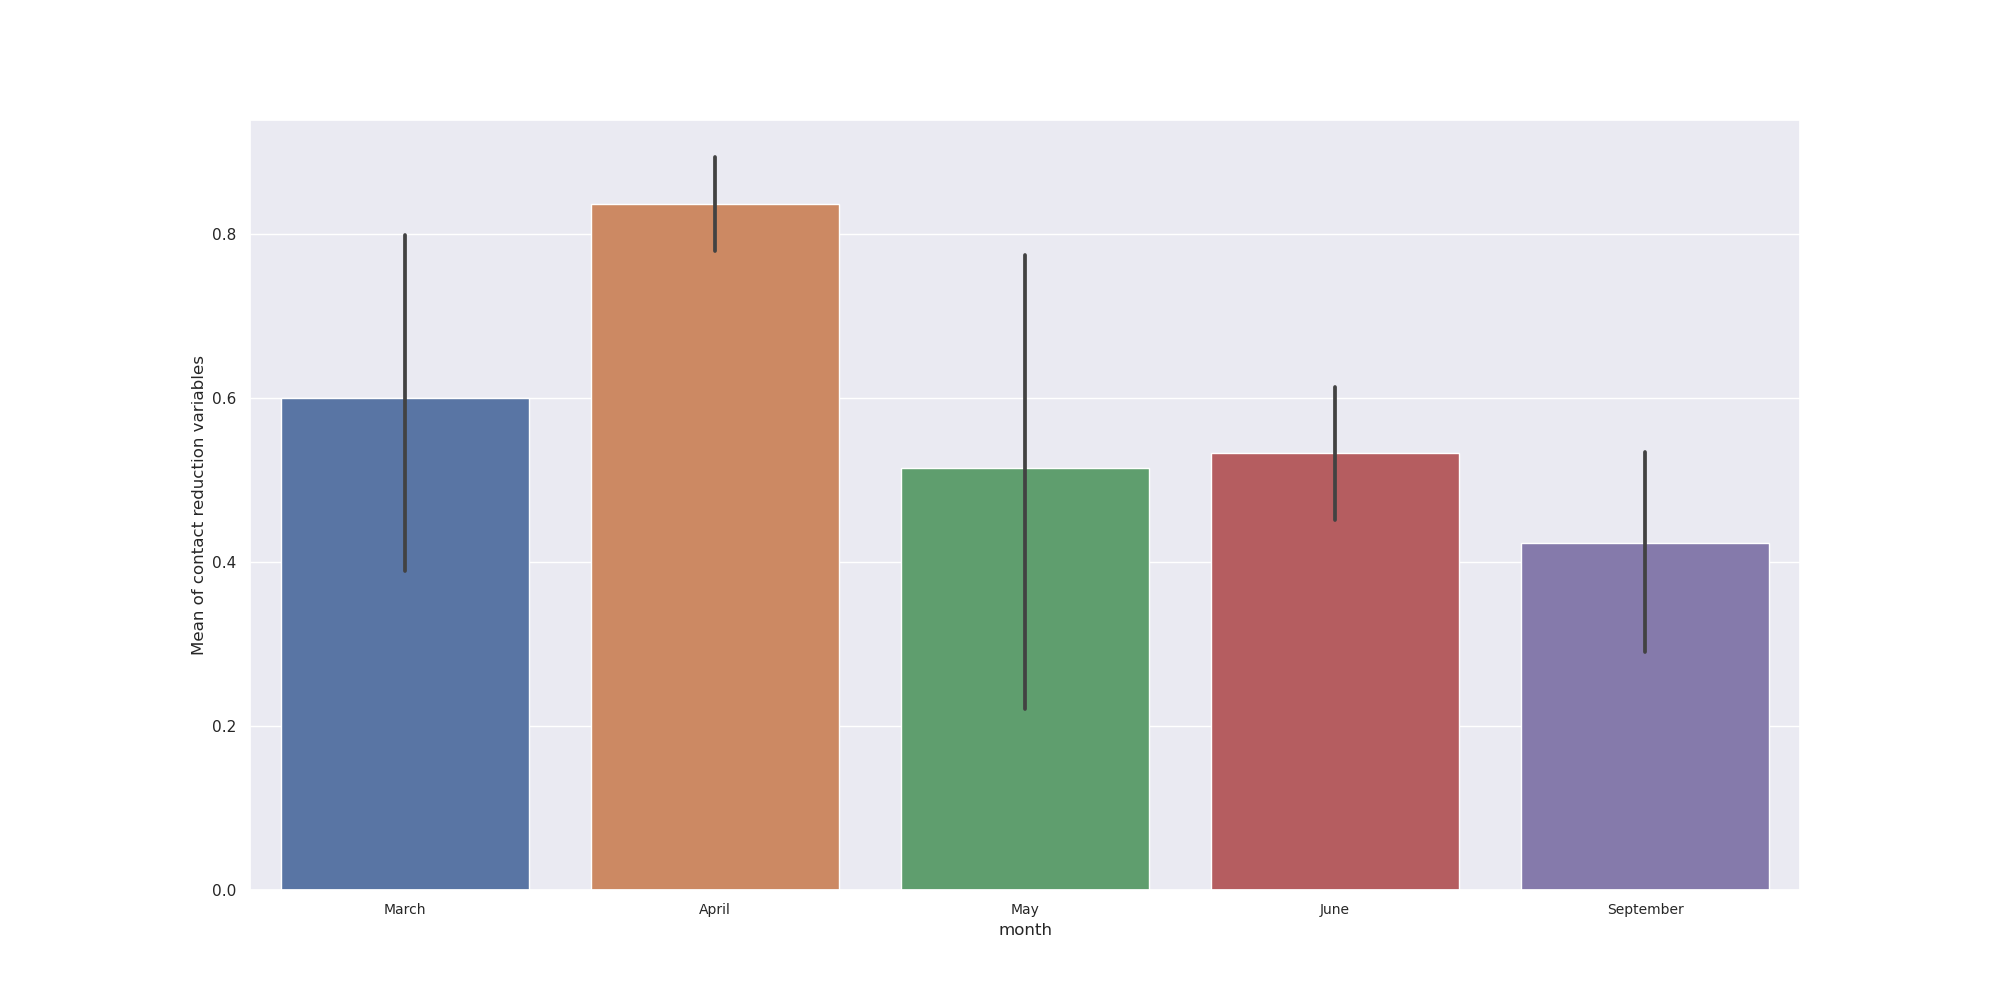
\includegraphics[width=\textwidth]{../../bld/figures/monthwise_mean_variables}
\end{figure}


\begin{figure}[H]
    \caption{Month-wise average of contact reduction variables}
    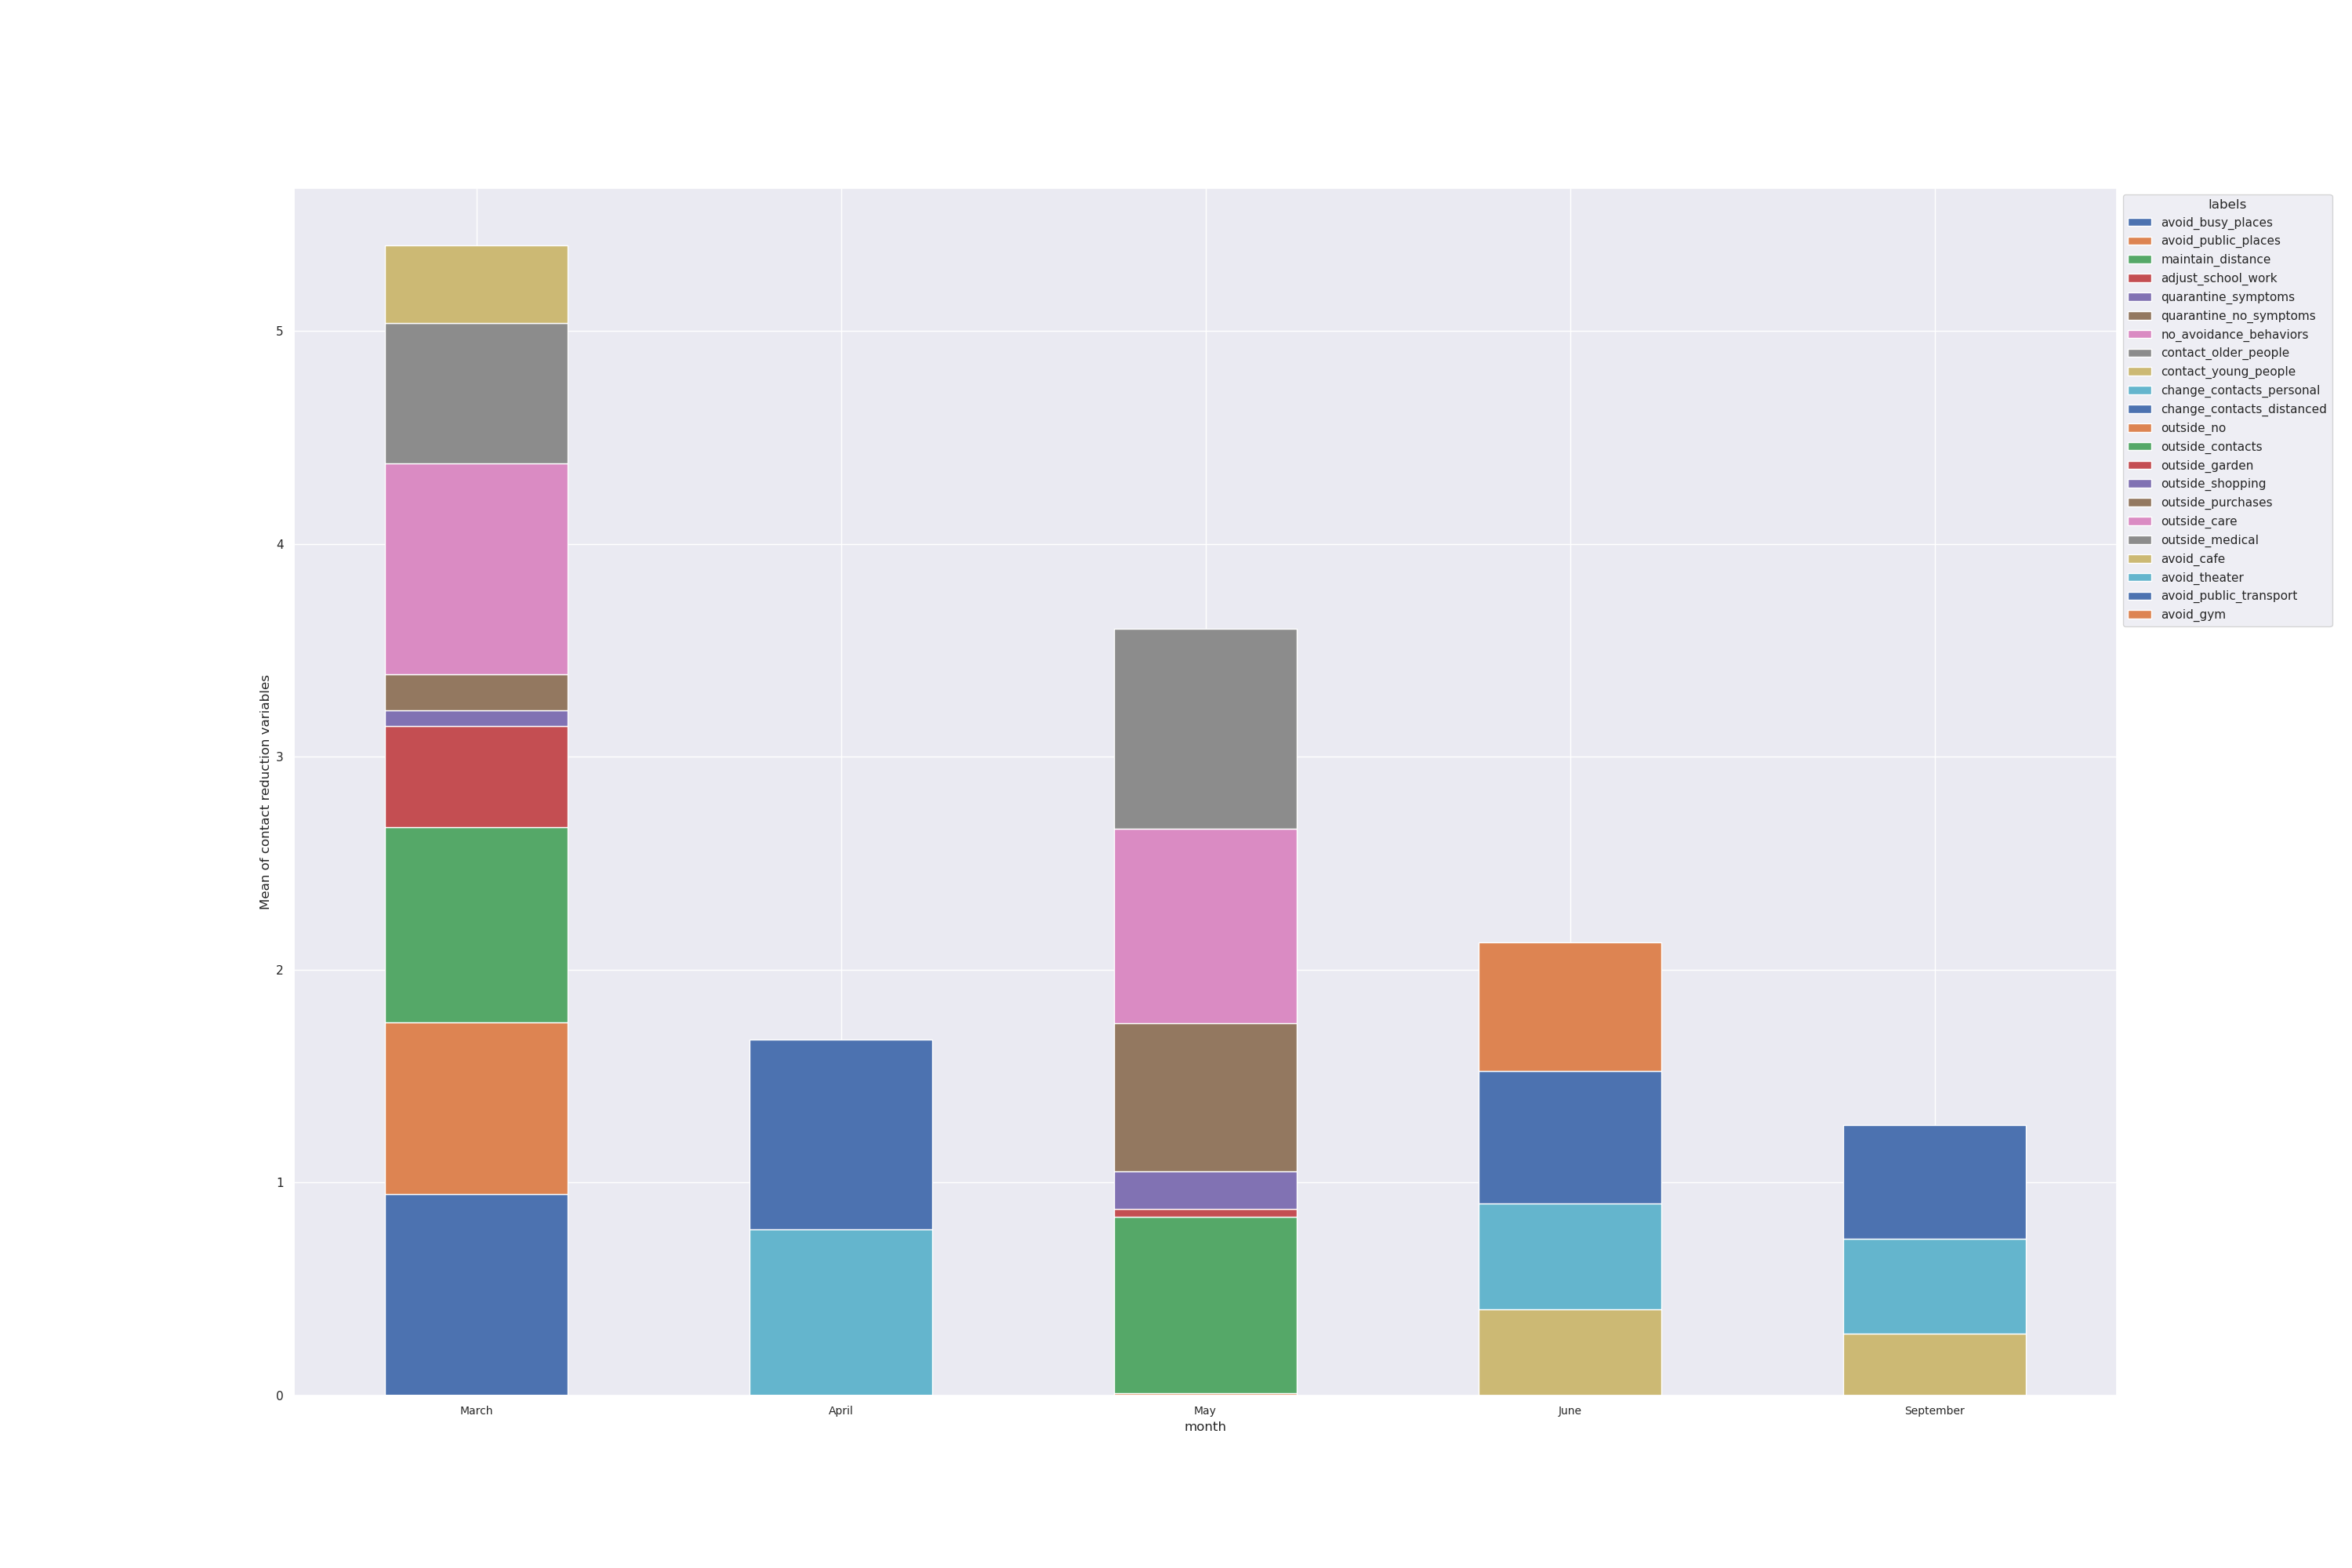
\includegraphics[width=\textwidth]{../../bld/figures/stackedbar}
\end{figure}


\newpage
\section{Incidence rate in Netherlands}

The information obtained from "Our World in Data" was restricted to data related to Netherlands. Previously the data set contained the incidence value per million population, however for our study we altered the incidence value per hundred thousand to attain the incidence value for the month in which the LISS panel survey was conducted. Figure 5 graphically represents the incidence value for the new cases and the total cases for the months beginning March 2020 to February 2020. Figure 6 plots the new cases, total cases and the incidence values for the new cases and the total cases. 


\begin{figure}[H]
    \caption{Time series incidence values for Netherlands}
    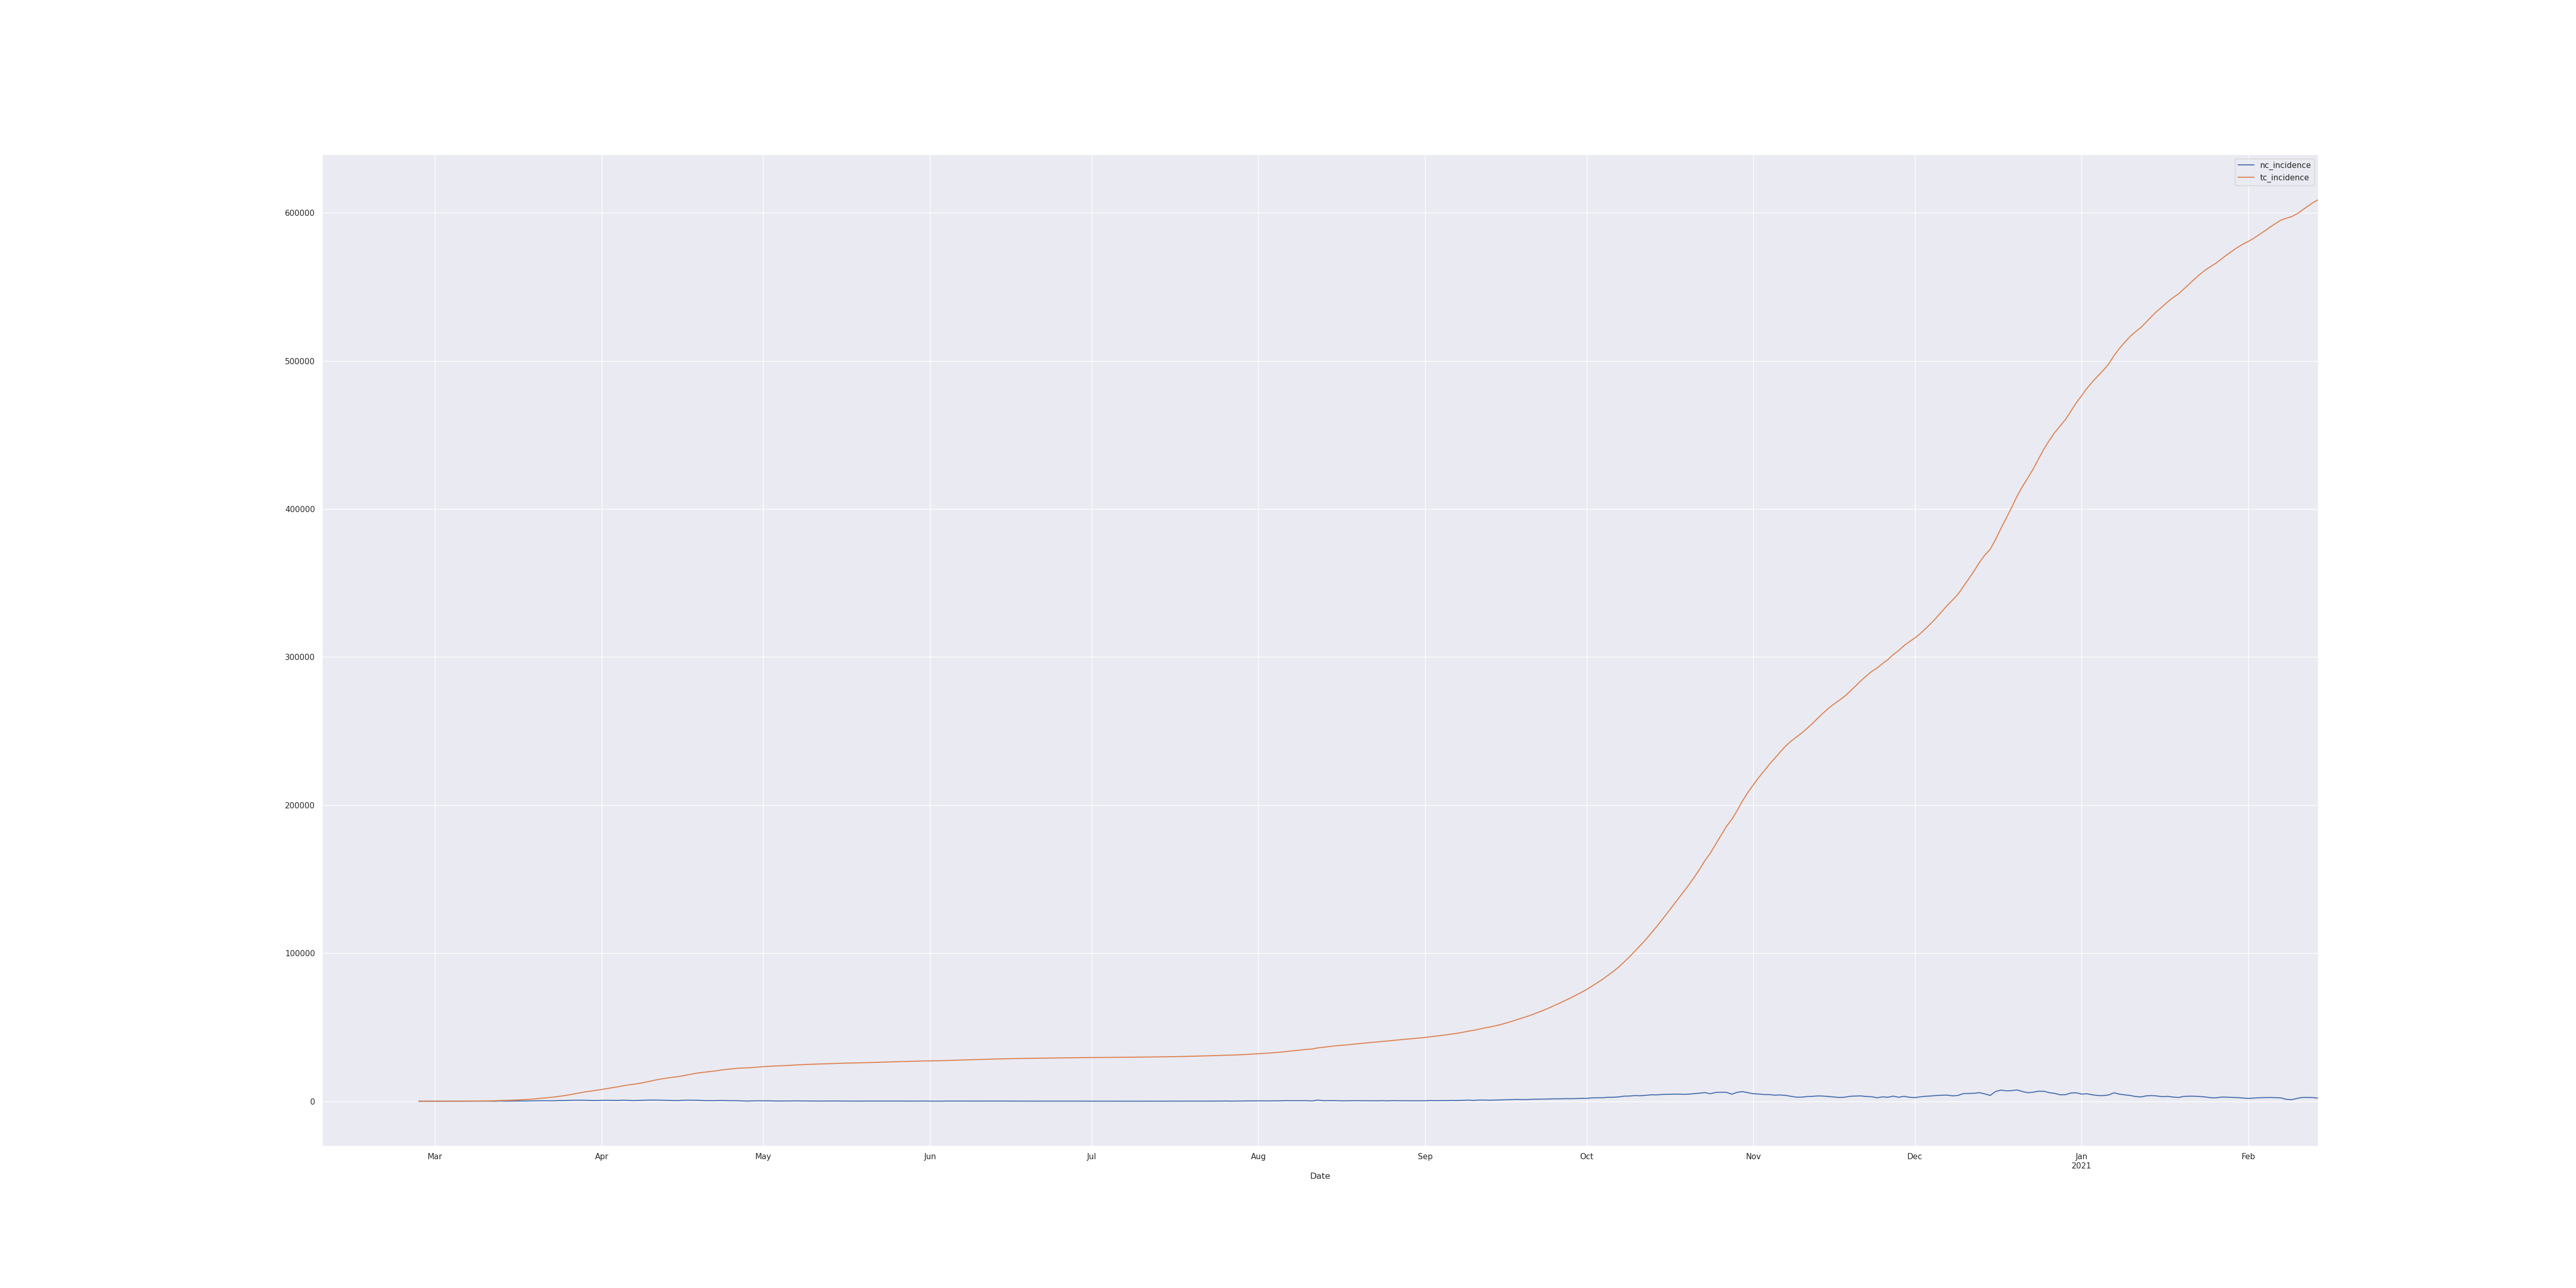
\includegraphics[width=\textwidth]{../../bld/figures/time_series}
\end{figure}

\begin{figure}[H]
    \caption{Time series incidence values for Netherlands}
    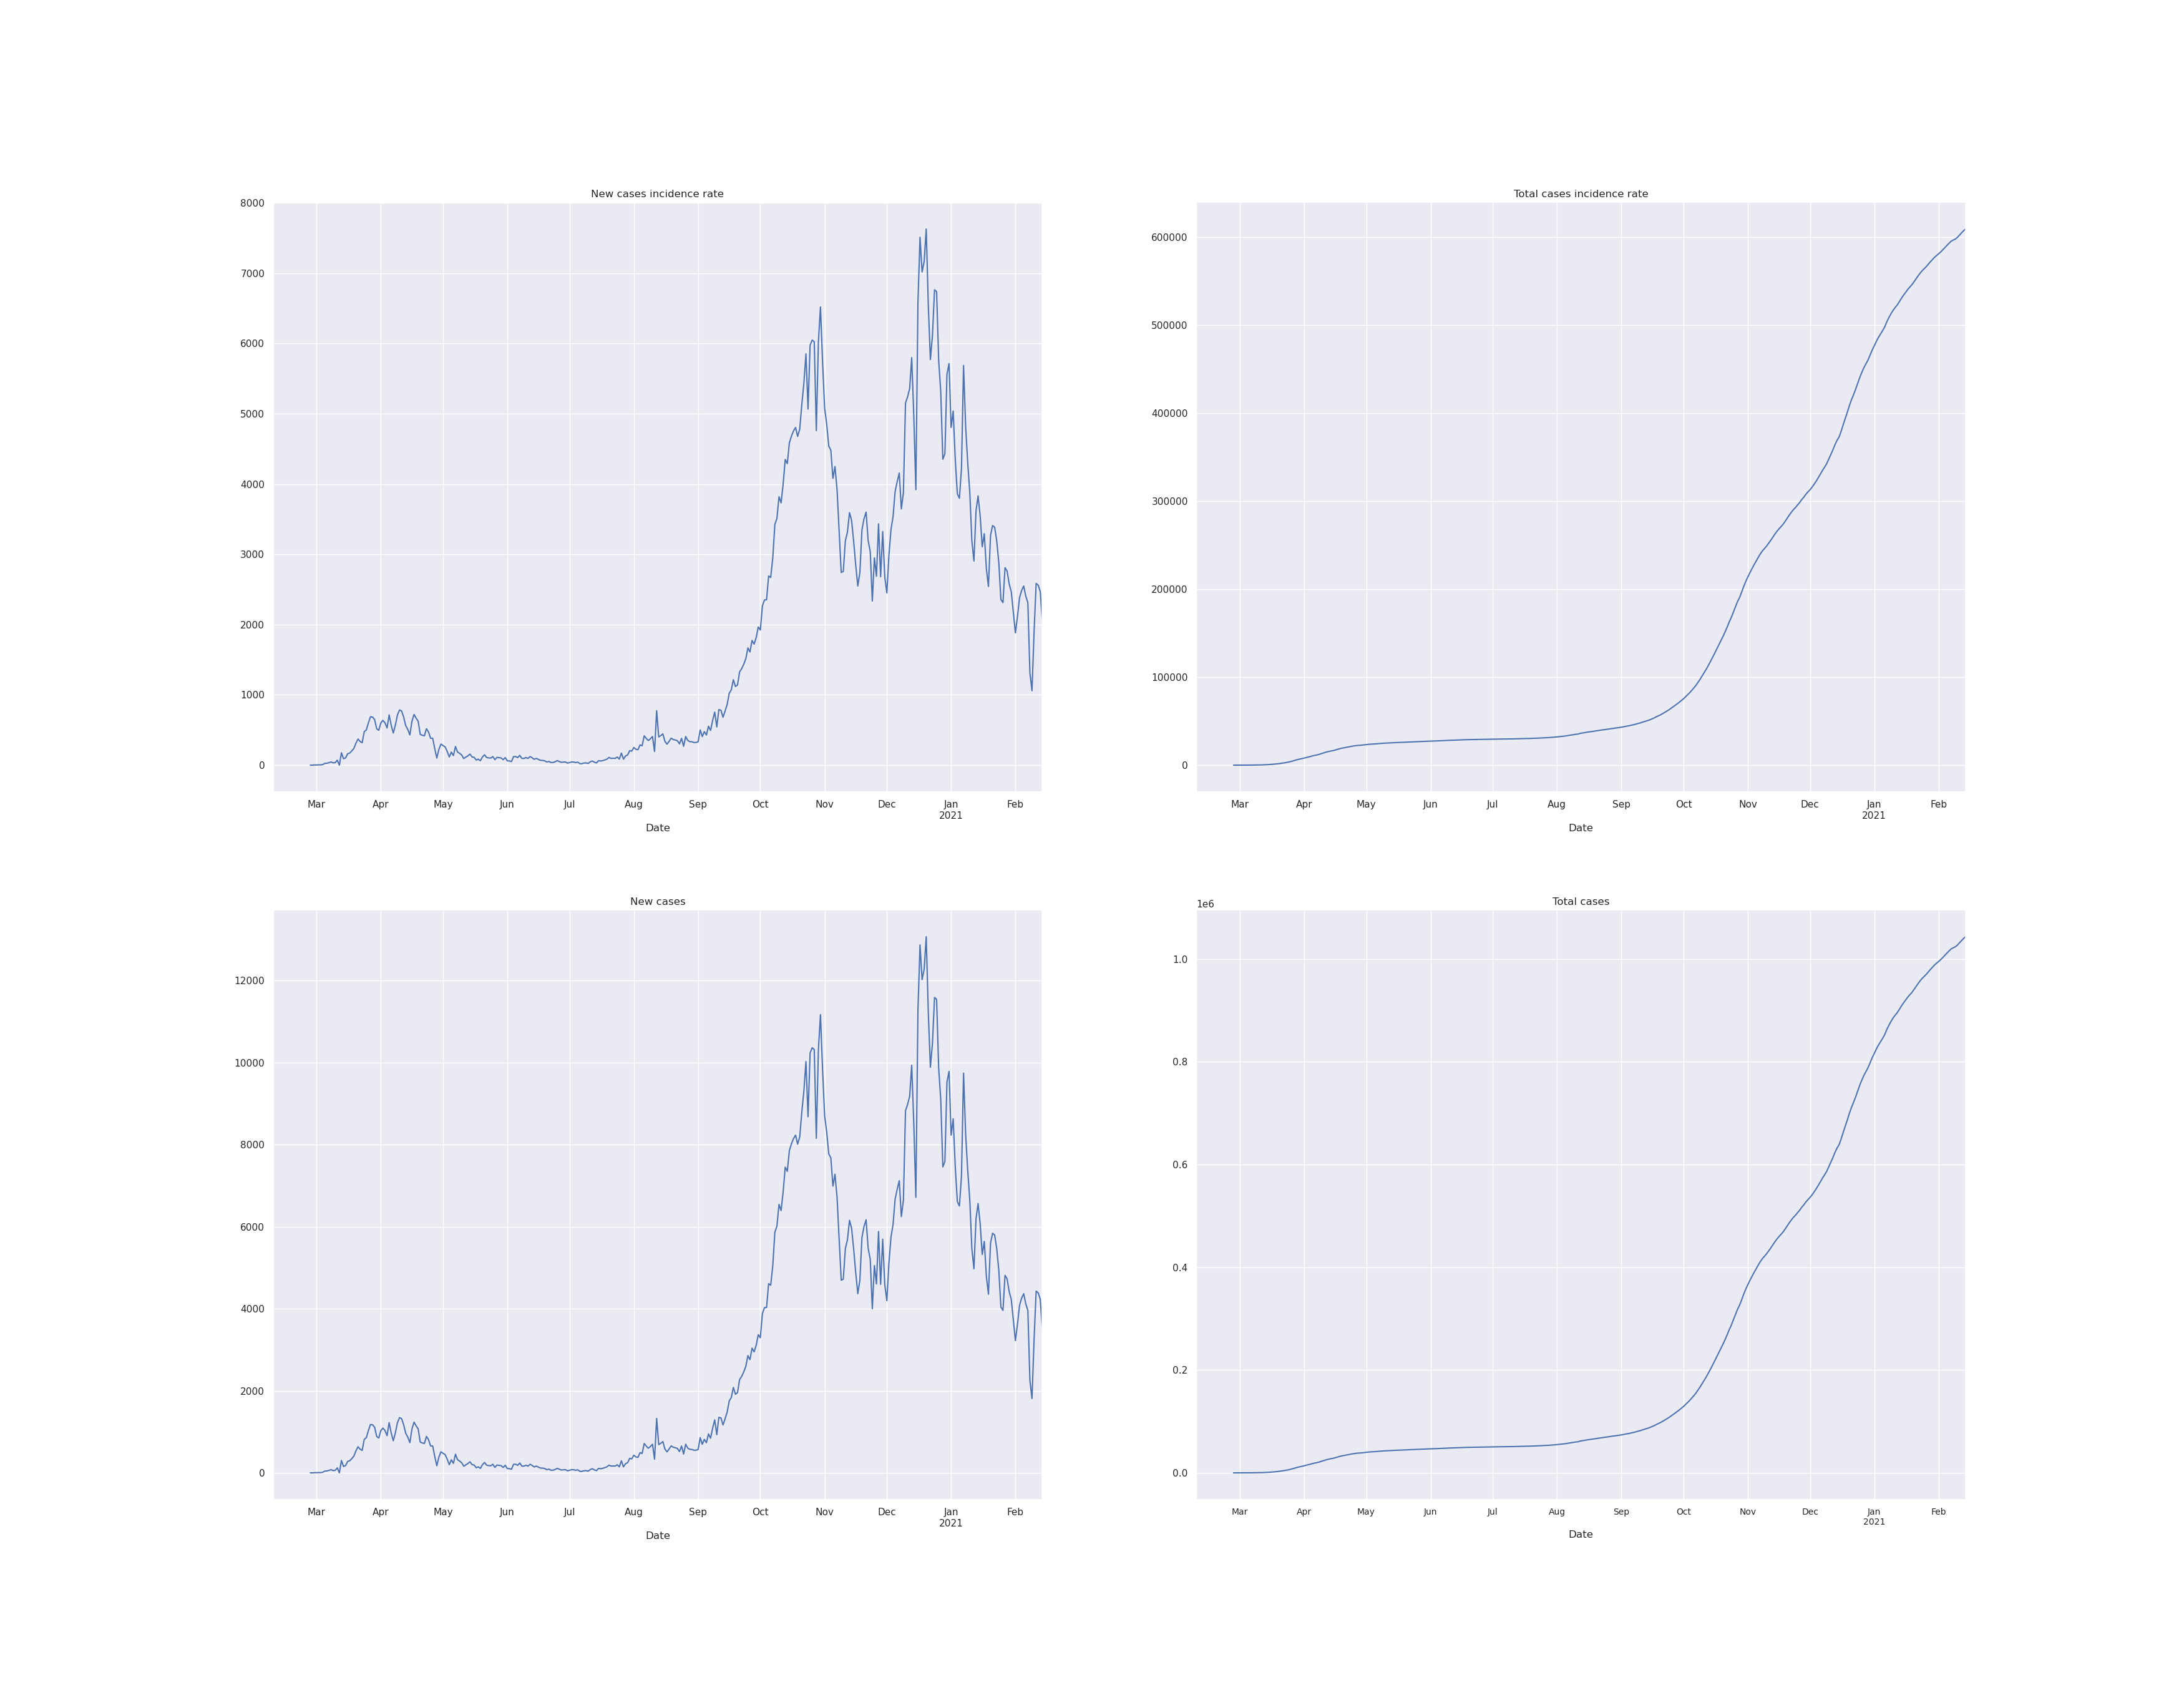
\includegraphics[width=\textwidth]{../../bld/figures/subplots}
\end{figure}





\newpage
\section{Results}
\subsection{Incidence rate and factors of contact reduction}

As we graphically present the association between our variables of interest related to contact reduction with the incidence value for new cases in the Netherlands we observe that our results are consistent with our  main assumptions for the the first four waves represented by the months of March, April, May and June. We find a reduction in contact amongst the population with an increase in the incidence value. However, for the fifth wave we observe lower levels of contact reduction with a peak in the incidence value. 

\begin{figure}[htp]
    \centering
    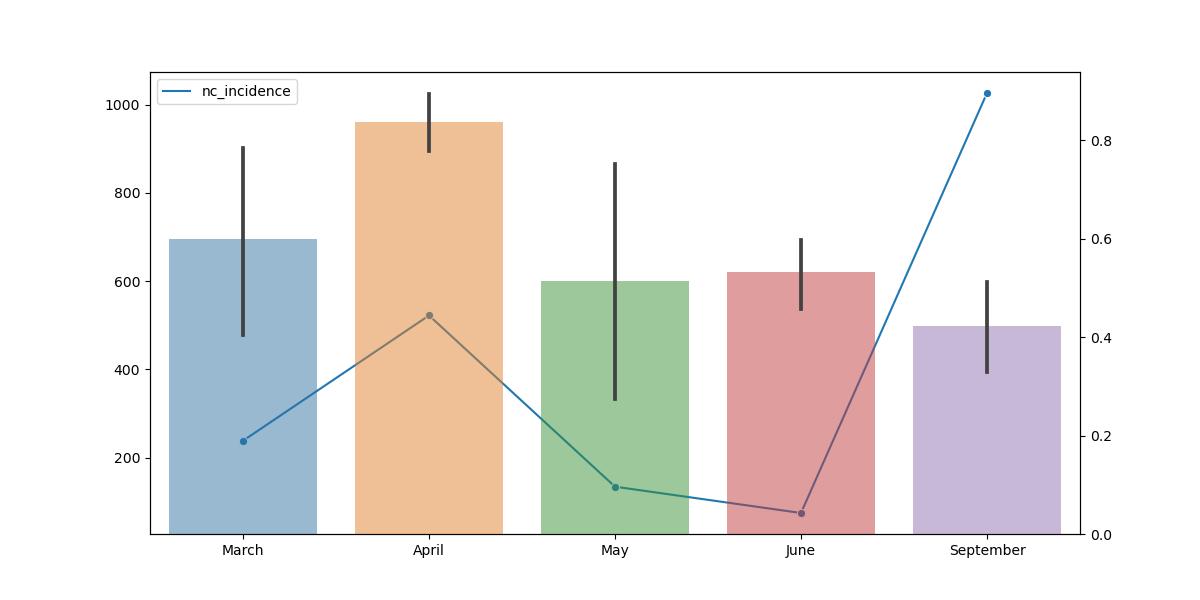
\includegraphics[width=12cm, height=10cm]{../../bld/figures/incidence_contact_reduction}
    \caption{}
    \label{fig:galaxy}
\end{figure}


\pagebreak
\subsection{OLS Results}
We have run the ordinary least square regression at two levels : wave-wise and across all the waves. We have taken the incidence value of new cases per hundred thousand population as the dependent(Y) variable and the contact reduction variables as the independent(X) variables. We have run the analysis using  logarithm of ``Y'' variable in order to observe the change of rate of new cases. However, due to very limited available data, the relevance of our OLS results is very limited. We have been able to achieve our set out objective of the aim of providing empirical evidence of an association between the incidence value and contact reduction graphically, however have not been able to yield statistical relevant OLS results. We discuss the importance of the results, observations and shortcomings in our approach.

 


\section{Discussion}
The OLS results across all the waves are interesting, especially the result with logarithm of new cases incidence value. It is statistically significant with almost all confidence intervals, however if we use some advanced techniques, for instance, a good instrumental variable then we can determine the direction of causality. We expect that with rise in new cases incidence value, people would become more cautious and their contact reduction behavior would rise. Thus, it is plausible that there is direct relationship between rise in CoViD-19 cases and rise contact reduction behavior by the individuals.

There are various shortcomings in the data. First of all, none of the variables are common in all the five waves, for these reasons we were unable to observe a variation in these variables over time. In the case if we had variables common for all the five waves we could provide a better estimation of which variables predict contact reduction accurately and measure the change over a specified period of time, this could be particularly useful for policymakers. 
Secondly, there are many missing values in the data which reduces the quality of data set substantially. Also, the OLS results of wave-wise analysis are not important because we have less number of observations then the number of independent variables. In the OLS analysis across all the waves, the results confirm the economic intuition but they are not sufficient to prove the causality. We propose that with similar data, we can find the causality by using better methods(instrument variable).


\begin{thebibliography}{9}
\bibitem{latexcompanion} 
Gaudecker Hans-Martin von. 
\textit{Templates for Reproducible Research Projects in Economics}. 
\texttt{https://doi.org/10.5281/zenodo.2533241}, 2019.

\bibitem{ourworldindata}
Max Roser, Hannah Ritchie, Esteban Ortiz-Ospina and Joe Hasell. \textit{Coronavirus Pandemic (COVID-19)". Published online at OurWorldInData.org.} 
\texttt{Retrieved from: 'https://ourworldindata.org/coronavirus' [Online Resource]}, 2020.

\bibitem{global} 
Hiscott, John and Alexandridi, Magdalini and Muscolini, Michela and Tassone, Evelyne and Palermo, Enrico and Soultsioti, Maria and Zevini, Alessandra
\textit{The global impact of the coronavirus pandemic}. 
Cytokine \& growth factor reviews, 53:1–9, 2020.

\end{thebibliography}




\end{document}